\documentclass[a4paper,slidestop,xcolor=pst,dvips,blue]{beamer}

\usepackage{beamerthemesplit}
\usepackage[utf8]{inputenc}
\usepackage[spanish]{babel}
\usepackage{graphicx}
\usepackage{pstricks} % PSTricks package
\usepackage{setspace}
\usepackage{multirow}
\usepackage{listings}
\usepackage{pgfpages}
\usepackage{hyperref}
\usepackage{etoolbox}
\usepackage{epstopdf}

\makeatletter
\patchcmd{\beamer@sectionintoc}{\vskip1.5em}{\vskip0.5em}{}{}
\makeatother

\setbeamercovered{dynamic}
\setcounter{tocdepth}{2}
\setbeamercolor{frametitle}{fg=black,bg=white}
\setbeamercolor{section in toc shaded}{fg=black}
\setbeamercolor{section in toc}{fg=red}
\setbeamercolor{subsection in toc shaded}{fg=black}
\setbeamercolor{subsection in toc}{fg=red}
\setbeamerfont{section in toc}{size=\small}
\setbeamerfont{subsection in toc}{size=\small}
\setbeamertemplate{section in toc shaded}[default][99]
\setbeamertemplate{subsection in toc shaded}[default][99]

\AtBeginSection[]
{\begin{frame}[c]
  \frametitle{Índice}
	\tableofcontents[currentsection,
        sectionstyle=show/shaded,
        subsectionstyle=hide]
\end{frame}}

\AtBeginSubsection[]
{\begin{frame}[c]
	\frametitle{Índice}
	\tableofcontents[
  		currentsection,
  		sectionstyle=shaded/shaded,
  		currentsubsection,
  		subsectionstyle=show/shaded/hide
		]
\end{frame}}

\setbeamercolor{frametitle}{fg=black,bg=white}

\setbeamertemplate{frametitle}{
	\begin{centering}
		\insertframetitle
		\par
	\end{centering}
}

\usetheme[secheader]{Boadilla} 

\title[Trabajo Eficaz en Equipo]{Técnicas de Trabajo Eficaz en Equipo \\
(Local y Remoto)}

\author[P. Sánchez]{\alert{Pablo Sánchez}}

\institute[ISTR]{
		   Dpto. Ingeniería Informática y Electrónica \\
		   Universidad de Cantabria \\
		   Santander (Cantabria, España) \\
		   \texttt{p.sanchez@unican.es}
}

\date{}

\begin{document}

\begin{frame}[c]
	\titlepage
	\begin{columns}
		\column{.5\linewidth}
			\centering 
\includegraphics[width=.33\textwidth,keepaspectratio=true]{images/istr.eps}
		\column{.5\linewidth}
			\centering
			
\includegraphics[width=.25\textwidth,keepaspectratio=true]{images/uc.eps}
	\end{columns}
\end{frame}

\section{Introducción}

\subsection{Objetivos}

\begin{frame}[c]
	\frametitle{Objetivo}
	\begin{block}{Objetivo}
		Adquirir habilidades de trabajo en equipo (local y remoto) de forma que éste resulte más eficaz y permita alcanzar mejores resultados que mediante el trabajo individual.
	\end{block}
\end{frame}

\subsection{Motivación}

\begin{frame}[c]
	\frametitle{Situación Idealizada Trabajo en Equipo}
	\begin{center}
		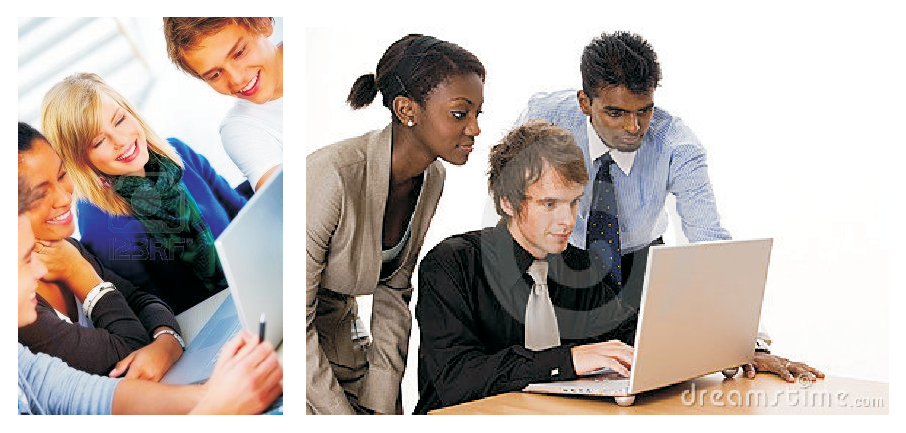
\includegraphics[width=\linewidth,keepaspectratio=true]{images/motivacion.eps}
	\end{center}
\end{frame}

\begin{frame}[c]
	\frametitle{Situación Real Trabajo en Equipo}
	\begin{center}
		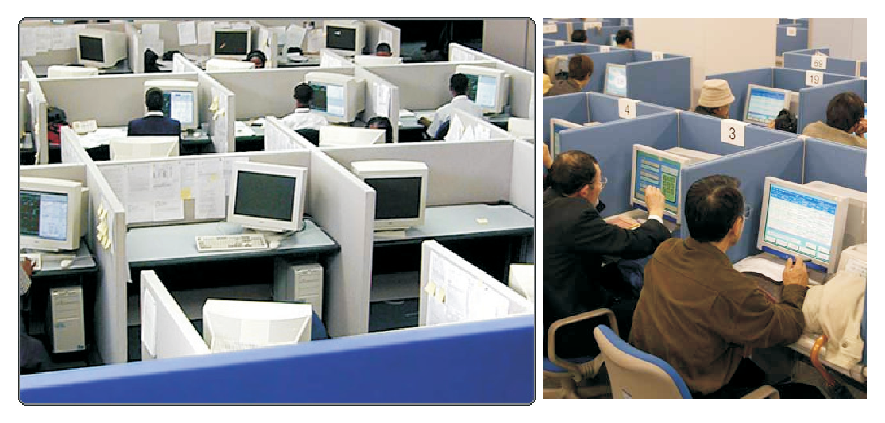
\includegraphics[width=\linewidth,keepaspectratio=true]{images/realidad.eps}
	\end{center}
\end{frame}

\begin{frame}[c]
	\frametitle{Tipos de Compañeros de Equipo}

    \renewcommand{\arraystretch}{2.0}   

	\begin{center}
		\begin{tabular}{|l|l|c|c|}
            \cline{3-4}
            \multicolumn{2}{l}{}  & \multicolumn{2}{|c|}{Capacidad de  Trabajo} \\ \cline{3-4}
            \multicolumn{2}{l|}{} &         Alta                 & Baja         \\ \cline{1-4}
            \multirow{2}{*}{\rotatebox[origin=c]{90}{Afinidad}} & \rotatebox[origin=c]{90}{Alta} & Unicornio & Colega Cañas \\ 
            \cline{2-4}
            & \rotatebox[origin=c]{90}{Baja} & Compañero Curro & Huir \\ 
            \cline{1-4} 
        \end{tabular}
	\end{center}
\end{frame}


\section{Fundamentos del Trabajo Eficaz en Equipo}

\subsection{Fundamento Trabajo Eficaz en Equipo}

\begin{frame}[c]
	\frametitle{Regla Fundamental para el Trabajo Eficaz en Equipo}
	\begin{block}{Regla Fundamental Trabajo en Equipo}
		Establecer claramente:
		\begin{itemize}
			\item<2-> El objetivo final que ha de satisfacer el equipo.
			\item<3-> Por qué trabajamos en equipo en lugar de individualmente.
		\end{itemize}
	\end{block}
\end{frame}

\subsection{Pautas para un Eficaz Trabajo en Equipo}

\begin{frame}[c]
	\frametitle{Estrategias de Trabajo Eficaz en Equipo}
	\begin{itemize}[<+->]
		\item Las tareas están claramente identificadas.
		\item La asignación de responsabilidades es clara.
		\item Las tareas son lo más autónomas posibles.
		\item Las dependencias entre tareas están claramente identificadas.
		\item Existen mecanismos de coordinación claramente definidos.
		\item No existen trabajadores ociosos.
		\item No existen trabajadores sobrecargados.
		\item No hay trabajadores infrautilizados ni sobrevalorados.
		\item Existen controles y revisiones de calidad.
		\item Hay tiempo para corregir defectos e imperfecciones si se detectasen.
	\end{itemize}
\end{frame}

\section{Técnicas para el Trabajo Eficaz en Equipo}

\subsection{Celebración de Reuniones}

\begin{frame}[c]
	\frametitle{Celebración de Reuniones}
	\begin{itemize}[<+->]
		\item En general, deben evitarse las reuniones.
		\item Establecer siempre cuál es el objetivo de la reunión.
		\item Elaborar una miniagenda para la reunión.
		\item Elaborar un simple acta para recordar que se acordó en la reunión.
		\item Elegir un moderador.
	\end{itemize}
\end{frame}

\subsection{Toma de Decisiones}

\begin{frame}[c]
	\frametitle{Toma de Decisiones}
	\begin{itemize}[<+->]
		\item La opinión de todo el mundo merece respeto.
		\item Acotar el tiempo necesario para tomar una decisión.
		\item Una decisión, una vez tomada, está tomada, salvo que se pruebe que es errónea.
		\item Las decisiones las toma todo el grupo y son responsabilidad de todo el grupo.
		\item Implantar algunos sistemas para decidir en caso de empate en votaciones (ej. voto doble).
	\end{itemize}
\end{frame}

\subsection{Controles de Calidad}

\begin{frame}[c]
	\frametitle{Controles de Calidad}
	\begin{itemize}[<+->]
		\item Todo material producido debe ser verificado por otro miembro del grupo distinto al que lo produjo.
		\item Debe verificarse con tiempo suficiente para reaccionar en caso de detectar defectos.
		\item Las tareas de verificación deben estar claramente establecidas y definidas.
		\item Aplicar la técnica del \emph{abogado del diablo} cuando corresponda.
		\item Si se ve que hay deficiencias en el propio proceso de trabajo en equipo, analizarlas y subsanarlas.
	\end{itemize}
\end{frame}

\subsection{Herramientas de Trabajo en Grupo}

\begin{frame}[c]
	\frametitle{Herramientas para Trabajo en Grupo}
	\begin{itemize}[<+->]
		\item Decidir herramientas y técnicas para compartir los artefactos que se generen (Git, Dropbox, OneDrive).
		\item Asegurarse de que las herramientas son compatibles (CRLF, UTF8, etc).
		\item Definir políticas para gestionar los artefactos comunes.
	\end{itemize}
\end{frame}

\section{Trabajo en Equipo Remoto}

\begin{frame}[c]
	\frametitle{¿Por qué tengo que trabajar en la empresa?}
	\begin{center}
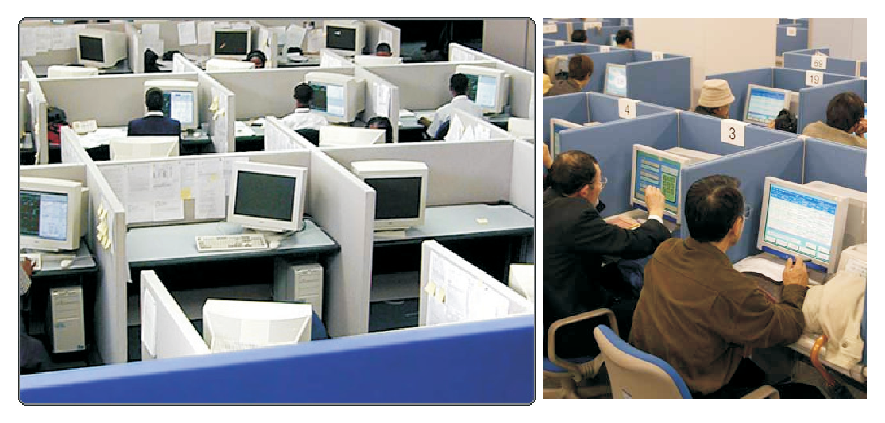
\includegraphics[width=\linewidth,keepaspectratio=true]{images/realidad.eps}
	\end{center}
\end{frame}

\begin{frame}[c]
	\frametitle{Justificaciones para el Trabajo Remoto}
	\begin{itemize}[<+->]
        \item Conciliación familiar o personal.
        \item Reducción de costes de personal.
        \item Implantación internacional.
        \item Miembros del equipo itinerantes.
	\end{itemize}
\end{frame}

\begin{frame}[c]
	\frametitle{Problemas del Trabajo Remoto}
	\begin{itemize}[<+->]
        \item Coordinación de horarios.
        \item Mantener la visión del grupo.
        \item Mantener el contacto y la calidez de la cercanía.
	\end{itemize}
\end{frame}

\begin{frame}[c]
	\frametitle{Principios para un Trabajo Remoto Eficaz}
	\begin{itemize}[<+->]
        \item Tareas lo más independiente posible.
        \item Tener reglas de trabajo claras.
        \item Usar herramientas asíncronas para mantener pequeñas interacciones y el contacto.
        \item Tener un mecanismo para hacer claras las decisiones.
        \item Usar teléfono y videoconferencia para mantener la interacción personal.
        \item Maximizar las \emph{golden hours}.
        \item En general, no perjudicar al trabajador presencial.
        \item \emph{Todos nosotros} vs \emph{locales y remotos}.
        \item \emph{Code reviews} para mantener la consistencia del producto.
	\end{itemize}
\end{frame}

%\begin{frame}[c]
%	\frametitle{Principios para un Eficaz Trabajo Remoto}
%	\begin{itemize}[<+->]
%        \item Tener un sitio donde publicar las decisiones globales (y sus justificaciones).
%        \item Políticas de gestión de problemas.
%        \item En general, no perjudicar al trabajador presencial.
%	\end{itemize}
%\end{frame}

\section{Conclusiones}

\begin{frame}[c]
	\frametitle{Conclusiones}
	\begin{itemize}[<+->]
		\item Trabajar en equipo no es trabajar todos juntos en el mismo sitio y a la misma hora.
		\item El trabajo en equipo debe ser eficaz. A nadie le gusta perder el tiempo.
		\item Un trabajo eficaz en equipo se basa en definir claramente un objetivo y diseñar una estrategia eficaz para satisfacerlo.
	\end{itemize}
\end{frame}

\end{document}
